\chapter{Tâche 2: Synthèse de l'ammoniac}

Dans cette tâche, il nous est demandé d'étudier la dernière étape
du procédé, c'est-à-dire la synthèse de l'ammoniac à partir de
gaz de synthèse, formé d'azote, d'hydrogène et d'argon.
Cette réaction est la réaction E sur la figure~\ref{fig:flowsheet2}.

Nous allons d'abord étudier les taux de conversion que nous pouvons obtenir
de façon théorique
dans le réacteur et déterminer s'il est possible de faire réagir l'entièreté
du \ce{N2} et du \ce{H2} présents,
en faisant varier la température et la pression.
Cette option n'étant pas réalisable,
nous allons proposer une solution de recyclage des réactifs pour
améliorer le rendement.
Ces calculs théoriques sont réalisés avec \matlab{}.

Ensuite, nous allons utiliser le logiciel \aspen{} pour modéliser le procédé
que nous proposons de manière plus précise,
et comparer les résultats obtenus.
Nous allons expliquer comment les hypothèses simplificatrices
ont faussé nos calculs théoriques, et comment il serait encore possible
d'améliorer la modélisation en prenant d'autres facteurs en considération.

\section{Approche théorique}

Dans cette sections nous allons étudier le processus de réaction-séparation
avec \matlab{}, d'abord sans recyclage, puis avec recyclage.

\subsection{Réaction seule}

Commençons donc par estimer le rendement que nous pourrions obtenir
sur cette dernière réaction:
\begin{equation}
    \label{eq:chem-e}
    \ce{N2 + 3H2 <-> 2NH3}
\end{equation}
Jusqu'à présent, dans la tâche 1, nous avions
considéré cette réaction comme complète.
Il faut donc maintenant résoudre les relations d'équilibre,
et étudier le résultat en fonction de la température et de la pression.

Pour cela, nous allons procéder comme pour les réactions du reformage primaire
en section~\ref{ssec:expr-eq}.
Soit $K\ind{E}$ la constante d'équilibre
de cette réaction. On a alors la relation:
\begin{equation}
    K\ind{E} = \frac{a_\ce{NH3}^2}{a_\ce{N2}\,a_\ce{H2}^3}
    = \frac{p_\ce{NH3}^2}{p_\ce{N2}\,p_\ce{H2}^3}
\end{equation}

Soient $\dot{n}_\ce{NH3}$, $\dot{n}_\ce{N2}$, $\dot{n}_\ce{H2}$
et $\dot{n}\ind{tot}$ les débits d'ammoniac, d'azote, d'hydrogène
et le débit total sortant du réacteur.
En exprimant les pressions partielles selon les fractions molaires
et la pression totale, on obtient:
\begin{equation*}
    K\ind{E} = \frac{(\dot{n}_\ce{NH3}\,/\,\dot{n}\ind{tot})^2
    \ \times (p\ind{tot}\,/\,p\ind{ref})^2}
    {(\dot{n}_\ce{N2}\,/\,\dot{n}\ind{tot})\ 
    (\dot{n}_\ce{H2}\,/\,\dot{n}\ind{tot})^3
    \ \times\ (p\ind{tot}\,/\,p\ind{ref})^4}
\end{equation*}
ou encore:
\begin{equation}
    \label{eq:equi-e}
    K\ind{E} \times (p\ind{tot}\,/\,p\ind{ref})^2
    = \frac{\dot{n}_\ce{NH3}^2\ \dot{n}\ind{tot}^2}
    {\dot{n}_\ce{N2}\ \dot{n}_\ce{H2}^3}
    = K_{\mathrm{E},\,p\indt{tot}}
\end{equation}

Soient $a$, $3a$ et $a/78$ les débits de \ce{N2}, \ce{H2} et \ce{Ar} entrants,
et soit $\epsilon$ le degré d'avancement de la réaction
(comme déjà défini dans la section~\ref{ssec:inco-eq}).
Alors, l'équation s'écrit encore:
\begin{equation*}
    K_{\mathrm{E},\,p\indt{tot}}
    = \frac{(2\epsilon)^2\,(4.013a-2\epsilon)^2}
    {(a-\epsilon)\,(3(a-\epsilon))^3}
\end{equation*}

De plus, si nous nommons $y$ le rapport $\epsilon / a$ de conversion
des réactifs, l'équation devient:
\begin{equation}
    K_{\mathrm{E},\,p\indt{tot}}
    = \frac{(2y)^2\,(4.013-2y)^2}{(1-y)\,(3(1-y))^3}
    = \frac{4y^2\,(4.013-2y)^2}{27(1-y)^4}
\end{equation}
on peut facilement la résoudre numériquement comme une recherche de racines
d'un polynôme de degré 4.

Si on prend les température et pression indiquées dans l'énoncé,
c'est-à-dire $T=750\,\kelvin$ et $p\ind{tot}=270\,\bbar$, on obtient un taux de conversion:
\begin{equation*}
    y = 0.4006
\end{equation*}
ce qui est assez médiocre: cela signifie que seuls $40\%$ des réactifs
réagissent effectivement, et $60\%$ sont simplement jetés,
après séparation dans une unité flash.

\subsubsection{Analyse paramétrique}

Nous allons maintenant étudier l'effet d'un changement
de température ou de pression sur le rendement de la réaction,
dans des intervalles réalistes.

\begin{figure}
    \centering
    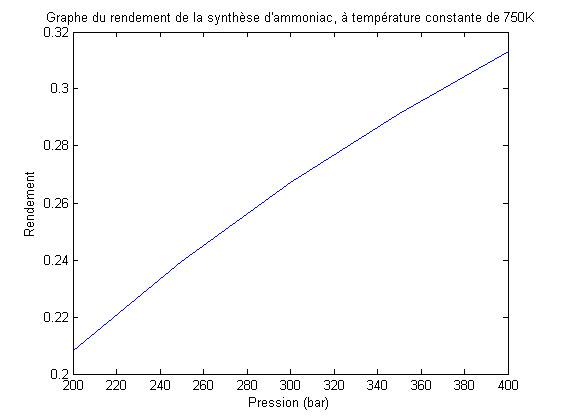
\includegraphics[width=0.8\textwidth]{img/param-press}
    \caption{
        Taux de conversion de la réaction de synthèse,
        pour $T=750\,\kelvin$.
        \emph{Augmenter la pression permet d'améliorer le rendement,
        mais c'est sans doute techniquement plus difficile et cher.}
    }
    \label{fig:param-press}
\end{figure}

Commençons par faire varier la pression entre $200\,\bbar$ à $400\,\bbar$, pour une température constante de $750\,\kelvin$.
On peut constater sur la figure~\ref{fig:param-press} que le rendement s'améliore quand la pression augmente. En effet, quand on analyse l'équation chimique de la synthèse d'ammoniac \eqref{eq:chem-e}, il y a moins de moles de gaz dans les produits que dans les réactifs, et donc augmenter la pression aidera la réaction à se déplacer vers les produits.

Mais nous allons voir que la pression n'a pas une aussi grande influence que la température sur la réaction chimique, car le rendement varie seulement d'une dizaine de pourcents en absolu pour une pression variant du simple au double.

\begin{figure}
    \centering
    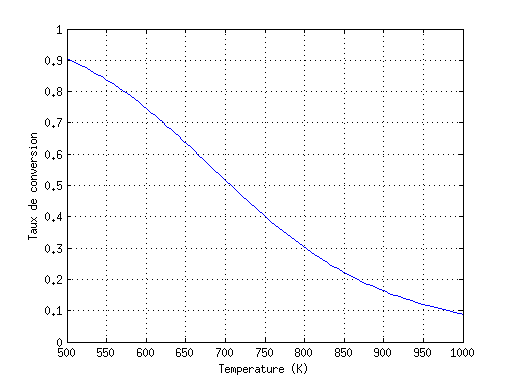
\includegraphics[width=0.8\textwidth]{img/param-temp}
    \caption{
        Taux de conversion de la réaction de synthèse,
        pour $p=270\,\bbar$.
        \emph{Baisser la température permet d'améliorer le rendement,
        mais la réaction va probablement devenir trop lente pour s'approcher
        de son équilibre.}
    }
    \label{fig:param-temp}
\end{figure}

Faisons maintenant varier la température entre $500\,\kelvin$ et $1000\,\kelvin$, pour une pression de $270\,\bbar$,
On peut observer dans la figure~\ref{fig:param-temp} que le rendement diminue quand la température augmente. En effet, comme il s'agit ici d'une réaction exothermique, au plus la température est élevée, au plus la réaction est favorisée vers les réactifs, ce qui diminue notre rendement.

On peut également constater que la température aura une plus grosse influence sur la réaction que la pression. Effectivement, on peut voir sur l'échelle des ordonnées que le rendement varie de plus de $80\%$ en absolu.

\subsubsection{Conclusions}

La conséquence de ces observations semble simple:
il faut augmenter la pression et baisser la température.
Toutefois, il faut prendre du recul et ne pas considérer uniquement
les équilibres chimiques.

En effet, augmenter la pression n'améliore pas sensiblement l'équilibre,
et cela ajouterait probablement des difficultés techniques, et par conséquent
des coûts supérieurs. Puisque il nous est difficile d'estimer ces coûts et leur
impact sur le prix de production, nous allons adopter dans nos calculs suivants
la pression standard qui nous est donnée de $270\,\bbar$.

Baisser la température améliore nettement l'équilibre,
et faire cela n'augmenterait a priori pas les coûts de production,
mais la cinétique chimique serait ici le facteur limitant:
en effet, en pratique, la réaction a besoin de plusieurs chambres
avec catalyseurs pour s'approcher de l'équilibre.
Diminuer la température ne peut qu'empirer le problème.
De nouveau, il est difficile d'en estimer précisément l'effet,
et les critères à optimiser nous sont inconnus.
Nous allons donc adopter la température donnée de $750\,\kelvin$.

\subsection{Recyclage des réactifs}

Dans la section précédente, nous avons vu que le rendement de la réaction
est assez mauvais, et que changer les conditions d'opération n'aide pas
vraiment à améliorer la situation.
Il nous faut donc une autre solution.

Cette solution consiste, après avoir séparé l'ammoniac produit
des réactifs restants dans l'unité flash,
à récupérer les réactifs ainsi isolés pour
qu'ils puissent réagir à nouveau.
Dans cette section, nous allons étudier l'influence de cette
mesure en considérant que la séparation est parfaite, c'est-à-dire que
l'intégralité de l'ammoniac est séparée, et qu'aucune quantité d'azote,
d'hydrogène ou d'argon n'est évacuée en même temps.

Remarquons directement que si tout est recyclé et réintroduit dans le
réacteur, l'argon ne sortira jamais du réacteur, et va s'accumuler
jusqu'à causer un accident ou du moins arrêter la production.
Il faut donc qu'une partie des réactifs isolés soit quand même
purgée, afin de garder la quantité d'argon à un niveau raisonnable.
Par conséquent, après l'\emph{unité flash} qui sépare l'ammoniac du reste,
il faudra un \emph{splitter} qui sépare le flux en deux,
avec une certaine part de purge.

\subsubsection{Choix des variables}

Étant donné que le calcul de l'équilibre avec recyclage est assez complexe,
commençons par présenter nos variables.
\begin{itemize}
    \item $a$ représente les débits molaires entrant dans le système,
        sans la partie recyclée; en particulier, arrivent dans le système
        des quantités
        $a$ de \ce{N2}, $3a$ de \ce{H2} et $a/78$ de \ce{Ar}.
    \item $b$ représente les débits molaire recyclé;
        en particulier, sont recyclées 
        des quantités $b$ de \ce{N2} et $3b$ de \ce{H2}.
        La quantité d'argon n'étant pas dans les mêmes proportions
        qu'à l'entrée, elle n'est pas donnée par la variable $b$.
    \item $c = a+b$ représente les débits molaires
        totaux entrant dans le réacteur;
        en particulier, arrivent dans le réacteur, avec réactifs frais et
        recyclés combinés des quantités
        $c$ de \ce{N2} et $3c$ de \ce{H2}.
        À nouveau, la quantité d'argon n'étant pas dans les mêmes proportions,
        elle sera traitée séparément.
    \item $\epsilon$ représente comme auparavant
        le degré d'avancement de la réaction;
        en particulier, $\epsilon$ de \ce{N2} et $3\epsilon$ de \ce{H2}
        seront transformés en $2\epsilon$ de \ce{NH3}.
    \item $r$ représente la fraction des réactifs séparés
        (\ce{N2}, \ce{H2} et \ce{Ar}) qui est recyclée et réinjectée
        dans le réacteur.
\end{itemize}

\subsubsection{Argon dans le réacteur}

Calculons maintenant la quantité d'argon qui entre dans le réacteur.
Pour rappel, avec le recyclage, l'argon s'accumule dans une certaine mesure,
qui dépend du rapport de recyclage: si rien n'est recyclé, il n'y a pas
d'accumulation; si tout est recyclé, l'argon s'accumule indéfiniment;
et dans les autres cas, il va s'accumuler jusqu'à atteindre un plafond.

Supposons que l'accumulation maximale d'argon est atteinte,
et donc qu'il est en quantité constante dans le système.
Puisqu'aucune quantité d'argon ne réagit, il faut,
selon l'équation~\ref{eq:gen-non-accu}, que le débit d'entrée d'argon soit égal
à son débit de sortie.

Soit $\dot{n}_\ce{Ar}$ le débit d'argon dans le réacteur.
Dans le système, par définition, il entre $a/78$ d'argon,
car le flux recyclé n'est pas une entrée au niveau du système.
Ce qui sort est la partie purgée, car l'argon ne sort pas par la sortie
principale avec l'ammoniac. Puisque une fraction $1-r$ du flux restant
est purgée, une quantité $(1-r)\,\dot{n}_\ce{Ar}$ d'argon sort du système.

Pour que l'argon ne s'accumule pas, il faut donc:
\begin{equation*}
    a/78 = (1-r)\,\dot{n}_\ce{Ar}
\end{equation*}
ce qui donne:
\begin{equation}
    \dot{n}_\ce{Ar} = \frac{a}{78(1-r)}
\end{equation}

On peut vérifier intuitivement ces résultats en considérant des cas
particuliers: pour $r=0$ on retombe au cas sans recyclage,
et le débit d'argon est simplement celui entrant, $a/78$;
tandis que pour $r=1$ l'expression est une division par zéro,
car l'argon s'accumule à l'infini.

\subsubsection{Expression de la partie fraîche des réactifs}

Nous désirons maintenant obtenir une expression
pour la partie fraîche $a$ en fonction
de la quantité de réactifs totale $c$, dans le but de tout exprimer
selon cette variable plus tard.

Pour ça trouvons d'abord une expression pour $b$.
Elle est assez simple à trouver. La partie recyclée vaut le débit
de réactifs sortant du réacteur, multipliée par le rapport de recyclage:
\begin{equation*}
    b = r(c-\epsilon)
\end{equation*}

Ensuite, il suffit de soustraire cette expression à $c$ pour trouver $a$:
\begin{equation}
    \label{eq:expr-a}
    a = c-b = c-r(c-\epsilon) = c\,(1-r) + r\epsilon
\end{equation}

\subsubsection{Expression de l'équilibre}

Pour exprimer la relation d'équilibre,
nous reprenons l'équation~\ref{eq:equi-e}.
Cette fois, les débits à la sortie de la réaction sont:
\begin{equation*}
    \left\{
    \begin{array}{ccl}
        \dot{n}_\ce{N2} &=& c-\epsilon \\
        \dot{n}_\ce{H2} &=& 3c-3\epsilon \\
        \dot{n}_\ce{Ar} &=& \frac{a}{78(1-r)} \\
        \dot{n}_\ce{N2} &=& 2\epsilon \\
        \dot{n}\ind{tot} &=&
        \dot{n}_\ce{N2}+\dot{n}_\ce{N2}+\dot{n}_\ce{N2}+\dot{n}_\ce{N2}
        = 4c + \frac{a}{78(1-r)} - 2\epsilon \\
    \end{array}
    \right.
\end{equation*}

En injectant ces résultats dans l'équation, on obtient:
\begin{equation*}
    K_{\mathrm{E},\,p\indt{tot}}
    = \frac{(2\epsilon)^2\,(4c + \frac{a}{78(1-r)} - 2\epsilon)^2}
    {(c-\epsilon)\,(3(c-\epsilon))^3}
\end{equation*}

Nommons maintenant $y$ le rapport $\epsilon/c$ de conversion des réactifs;
cela nous permet de transformer l'équation en:
\begin{equation*}
    K_{\mathrm{E},\,p\indt{tot}}
    = \frac{(2y)^2\,(4 + \frac{a}{78c\,(1-r)} - 2y)^2}
    {(1-y)\,(3(1-y))^3}
\end{equation*}

Remplaçons maintenant $a$ par son expression en~\ref{eq:expr-a}:
\begin{equation*}
    K_{\mathrm{E},\,p\indt{tot}}
    = \frac{(2y)^2\,(4 + \frac{c\,(1-r) + r\epsilon}{78c\,(1-r)} - 2y)^2}
    {(1-y)\,(3(1-y))^3}
    = \frac{4y^2\,[(4 + \frac{1}{78}) + (\frac{r}{78(1-r)} - 2)y]^2}
    {27(1-y)^4}
\end{equation*}

À nouveau, cette équation est facilement résolvable numériquement
comme la recherche de racines d'un polynôme de degré 4,
ce qui donne la valeur de $y$ en fonction du paramètre $r$.

\subsubsection{Taux de conversion effectif}

Nous avons donc maintenant une valeur pour $\epsilon/c$.
Toutefois, cette valeur ne tient en compte qu'un cycle du réacteur:
ce qui est réellement consommé n'est pas $c$, mais bien $a$.
Dès lors, il faut passer de $y = \epsilon/c$ à $y\ind{eff} = \epsilon/a$.

Pour ce faire, calculons le rapport entre $a$ et $c$
en réutilisant l'équation~\ref{eq:expr-a}:
\begin{equation}
    \frac{a}{c} = \frac{c\,(1-r) + r\epsilon}{c} = (1-r) + ry
\end{equation}

On obtient donc:
\begin{equation}
    y\ind{eff} = y / (a/c) = \frac{y}{(1-r) + ry}
\end{equation}
ce qui nous donne le taux de conversion effectif
en tenant compte du recyclage.
On remarque que quand $r=0$, ce taux vaut simplement $y$,
tandis que quand $r$ tend vers 1, il tend vers 1 aussi.

Sa valeur pour différentes fractions de recyclage est présentée dans
le tableau~\ref{tab:result-theory}.

\begin{table}
    \centering
    \begin{tabu}{c|ccccccccccc}
        $r$ & 0.0 & 0.1 & 0.2 & 0.3 & 0.4
        & 0.5 & 0.6 & 0.7 & 0.8 & 0.9 & 1.0 \\
        \hline
        $y\ind{eff}$ & 0.40 & 0.43 & 0.46 & 0.49 & 0.53
        & 0.57 & 0.63 & 0.69 & 0.77 & 0.87 & N/A \\
    \end{tabu}
    \caption{Le taux de conversion effective tend vers 1 quand le
    rapport de recyclage augmente.}
    \label{tab:result-theory}
\end{table}

\section{Modélisation avec \aspen}

Pour modéliser le processus avec \aspen, nous avons utilisé
les composants suivants:
\begin{itemize}
    \item un compresseur isentropique, pour amener les réactifs à la pression
        de $270\,\bbar$;
    \item un préchauffeur, pour amener les réactifs à la température
        de $750\,\kelvin$;
    \item un réacteur à l'équilibre, pour simuler les réactions;
    \item un refroidisseur, pour refroidir les produits sortant du réacteur
        à la température de $250\,\kelvin$ propice à condenser l'ammoniac;
    \item une unité flash, pour séparer l'ammoniac du reste;
    \item et un splitter, pour partager le flux restant en un flux de recyclage
        et un flux de purge.
\end{itemize}

\begin{figure}
    \centering
    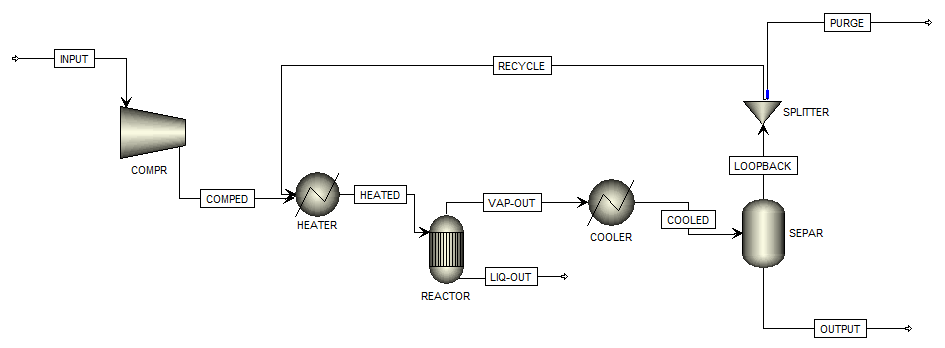
\includegraphics[width=\textwidth]{img/aspen}
    \caption{
        Flow-sheet de la modélisation réalisée sur \aspen.
    }
    \label{fig:aspen}
\end{figure}

La disposition de ces différents éléments et des flux les reliant
est donnée dans la figure~\ref{fig:aspen}. Deux remarques sur cette disposition:
\begin{itemize}
    \item Le flux \textsc{recycle} est réinséré avant le bloc \textsc{heater}.
        En effet, puisqu'il sort du séparateur, il est à $250\,\kelvin$
        et a donc besoin d'être réchauffé avant d'entrer dans le réacteur.
    \item Le flux \textsc{liq-out} liquide sortant du réacteur est juste là pour
        remplir les exigences du programme. Étant donné la température de
        $750\,\kelvin$ régnant dans dans le réacteur, un fraction tout à fait
        négligeable des composés présent est sous forme liquide et le flux
        \textsc{liq-out} est vide pour la précision de la modélisation.
\end{itemize}

En faisant tourner la simulation pour plusieurs valeurs du rapport
de recyclage $r$, nous avons obtenus des valeurs pour le taux de conversion,
que nous avons indiqué dans le tableau~\ref{tab:result-aspen}

\begin{table}
    \centering
    \begin{tabu}{c|ccccccccccc}
        $r$ & 0.0 & 0.1 & 0.2 & 0.3 & 0.4
        & 0.5 & 0.6 & 0.7 & 0.8 & 0.9 & 1.0 \\
        \hline
        $y\ind{eff}$ & 0.41 & 0.43 & 0.46 & 0.49 & 0.53
        & 0.58 & 0.63 & 0.69 & 0.77 & 0.87 & N/A \\
    \end{tabu}
    \caption{Le taux de conversion effective tend vers 1 quand le
    rapport de recyclage augmente.}
    \label{tab:result-aspen}
\end{table}

\section{Comparaison des résultats}

Pour comparer les simulations faites avec \matlab{} et avec \aspen{},
nous avons étudié deux critères:
le taux de conversion effectif de la réaction (la quantité d'ammoniac
produite pour l'azote et l'hydrogène entrant dans le système)
et le débit à l'intérieur du réacteur pour une certaine quantité d'ammoniac
produite.
Nous avons calculé ces deux valeurs pour différents rapports de recyclage.
